%
% Settings file
%
% This template is based on the UiB PhD thesis template
%

\include{settings}	% Document settings file

%
% We use the book class
%

\documentclass[10pt]{book}
\renewcommand{\bibname}{References}
%
% The geometry package allows consistent control of page layout
%

% \usepackage[paper = a4paper,         %To be shrunk to 80% when printed
% 			oneside,                 %Two-side mode, switches margins 
% 			bindingoffset = 2mm,     %Offset for binding side of page
% 			hmargin = 25mm,          %Left and right margin
% 			vmargin = 25mm,          %Top and bottom margin
% 			dvipdfm]{}
% % 			{geometry}

% \usepackage[paper = a4paper,oneside,bindingoffset = 2mm,hmargin = 25mm,vmargin = 25mm,dvipdfm]{geometry}
\usepackage[a4paper, total={6in, 8in}]{geometry}
\usepackage{float}
\usepackage[T1]{fontenc}	% Activate Type 1 fonts
\usepackage{mathptmx}       % Use Times font, also for math
\usepackage[scaled]{helvet} % for sans serif fonts (\textsf{...} or \sffamiliy)
\usepackage{sectsty}        % Change section and chapter header
%\allsectionsfont{\usefont{T1}{phv}{bc}{n}\selectfont} % Set chapter/section header to narrow helvectica (arial-like)
%\usepackage[scaled]{luximono} % for monospaced fonts (\texttt{...} or \ttfamily)
\usepackage[numbers,sort&compress]{natbib}
\usepackage{titlesec}

%
% Packages we need
%
\usepackage{graphicx}       % Handles figures
\graphicspath{{./}{images/}{Docs/images/}{figures/}}
\usepackage[utf8]{inputenc} % We want æøå
\usepackage{amsmath}
\usepackage{amsfonts}
\usepackage[mathcal]{euscript} % For calligraphy fonts
\usepackage{booktabs}       % Publication quality tables
\usepackage{algorithm}
\usepackage{algorithmic}
\usepackage{multirow}
\usepackage{setspace}       % Easy setting of line spacing
\usepackage{forloop}		% For-loops!
% \usepackage[round]{natbib}  % author and names
%\usepackage[numbers,sort&compress]{natbib}  % Sort numerical keys for multiple cites
      % Avoid breaking 'backref' option of hyperref package   % named colors
% \usepackage[procnames]{listings} % beautiful listings
% \usepackage{units}				 % semantically represent numbers with units
% \usepackage{natbib}  
\usepackage[table]{xcolor}
\usepackage[final]{pdfpages}
\usepackage{epigraph}			%for quotation
\setlength\epigraphwidth{8cm}
%\setlength\epigraphrule{0pt} %remove line in quote
\usepackage{textcomp}
\usepackage{sidecap} %for figure caption on the side
\usepackage{enumitem} % for possibility to adjust item left margin indentation

\usepackage{titlesec} %fix header fonts
\titleformat{\title}[display]
  {\normalfont\rmfamily\huge\bfseries\color{black}}
  {\chaptertitlename\ \thechapter}{16pt}{\Huge}
\titleformat{\chapter}[display]
  {\normalfont\rmfamily\huge\bfseries\color{black}}
  {\chaptertitlename\ \thechapter}{16pt}{\Huge}
\titleformat{\section}
  {\normalfont\rmfamily\Large\bfseries\color{black}}
  {\thesection}{1em}{}
\titleformat{\subsection}
  {\normalfont\rmfamily\Large\bfseries\color{black}}
  {\thesubsection}{1em}{}


% The hyperref package allows advanced hyperlinking functionality
%
\usepackage[%dvipdfmx,        % Use dvipdf driver %KD removed
			backref,         % List citing occurences in the References
			colorlinks,      % Colored links
			citecolor=black,  % Color of cite links
			linkcolor=black,  % Color of links
			urlcolor=blue,   % Color of urls
			]{hyperref}
%\newcommand{\aref}[1]{\autoref*{#1}} % Prevent links
\newcommand{\aref}[1]{\autoref{#1}} % Enable links


%
% Set fancy page header using fancyhdr package
% 
\usepackage{fancyhdr}
\pagestyle{fancy}

% Ensure that the chapter and section headings are in lowercase
\setlength{\headheight}{13pt}
\renewcommand{\chaptermark}[1]{\markboth{#1}{}}
\renewcommand{\sectionmark}[1]{\markright{\thesection\ #1}}

% Delete current section for header/footer
\fancyhf{}

% Define header/footer layout
\fancyhead[LE,RO]{\bfseries\thepage}
\fancyhead[LO]{\bfseries\rightmark}
\fancyhead[RE]{\bfseries\leftmark}
\renewcommand{\headrulewidth}{0.5pt}

% make space for the rule
\fancypagestyle{plain}{
    \fancyhf{}
    \renewcommand{\headrulewidth}{0pt}
}

\usepackage[font={small,it,rm}]{caption}
\usepackage{atveryend}
\usepackage{listings}
%\usepackage{thumbs}


%
% Set header height to 30pt to make room for two rows in the header
% (useful if you have very long chapter names)
%
%\headheight 30pt


%
% Include user-defined macros
%
\include{macros}

%
% TeX is very proud of its hyphenation engine, to the point where it 
% hyphenates _everything_ just to show off.  Increasing penalty for 
% hyphenation, and increase tolerance for underfull boxes can make 
% the text easier to read, at the expense of making the text less aligned
% to the right margin
%
\hyphenpenalty=10
\tolerance=1000


% Redefine include command -> input command
%\renewcommand{\include}{\input}

% Include only these chapters
%\includeonly{introduction}


%
% Set up the frontpage, with author, title, etc
%
%{\fontsize{28}{30}\usefont{OT1}{phv}{bc}{n}\selectfont 
%{\fontsize{28}{30}\usefont{T1}{phv}{bc}{n}\selectfont Exchange of water masses
\title{{\fontsize{19}{18}\sffamily\textbf{Federated Prototype Learning with Privacy-Aware Multi-Metric Client Selection for Software Defect Prediction}}
	\author{
\begin{minipage}[t]{0.4\textwidth}
\begin{flushleft} \large
\emph{Authors:}\\
Merugu Pavan Kalyan\\
Chandu Cherupally\\
Beernelly Sravan
\end{flushleft}
\end{minipage}
\begin{minipage}[t]{0.4\textwidth}
\begin{flushright} \large
\emph{Supervisor:} \\
Dr.~Manjubala Bisi
\end{flushright}
\end{minipage}
	    \vspace{5em}\\
		
\includegraphics[width=40mm]{uglo.png}\vspace{4em}\\
		A Dissertation Report\\
		Final Semester PROJECT WORK for B.Tech \\
		Department of Computer Science and Engineering \\
		NIT Warangal}
	\huge\date{\today}
}
\let\cleardoublepage\clearpage

% \setcounter{secnumdepth}{3}
%====================================================
%------------------ BEGIN DOCUMENT ------------------
%====================================================
\begin{document}
%Cause all references in bibtex file to appear in the 'References' section, even
%if they are not explicitly cite'ed in the document
%\nocite{*}

%Set the fontsize and baselineskip, if something other than 10 or 12 is required
\ifDownscaledFinalDoc
	\fontsize{\TextSize}{\BaseLineSkip}
	\selectfont
\fi

%Double line spacing for draft
\ifDraft
	\doublespacing
\fi

\renewcommand{\familydefault}{\sfdefault} %KD

%--------------------------------------------------------------------------------------------------
% FRONT MATTER
%--------------------------------------------------------------------------------------------------
\let\cleardoublepage\clearpage
\frontmatter
\let\cleardoublepage\clearpage
\normalfont\rmfamily

\thispagestyle{empty}

\begin{titlepage}
\begin{center}

{\bfseries\huge 
Federated Prototype Learning with Privacy-Aware Multi-Metric Client Selection for Software Defect Prediction}\\[1.2cm]

{\Large Submitted in fulfilment of the requirements for the degree of}\\[0.3cm]
{\Large \textbf{Bachelor of Technology} by}\\[0.2cm]

{\Large \textbf{Merugu Pavan Kalyan} (22CSB0A19)}\\[0.5 cm]
{\Large \textbf{Chandu Cherupally} (22CSB0C20)}\\[0.5 cm]
{\Large \textbf{Beernelly Sravan} (22CSB0A07)}\\[0.5 cm]

{\Large Supervisor:}\\[0.2cm]
{\Large \textbf{Dr Manjubala bisi}}\\[0.2cm]
{\large Assistant Professor, Department of CSE}\\[1.5cm]


\includegraphics[width=4.0cm]{uglo.png}\\[1.5cm]

{\Large \textbf{Department of Computer Science and Engineering}}\\[0.4cm]
{\Large National Institute of Technology, Warangal}\\[0.3cm]
{\Large India}\\

\vfill
{\Large \textbf{April 2026}}

\end{center}
\end{titlepage}
\chapter*{Acknowledgement}
\addcontentsline{toc}{chapter}{Acknowledgement}
I would like to express my heartily gratitude towards  \textbf{Dr Manjubala Bisi} for her valuable guidance, supervision,
suggestions, encouragement and the help throughout the semester, for the completion of my project work. She kept me going when I was down and gave me the courage to keep moving forward.

I also want to thank evaluation committee for their valuable suggestions and conducting smooth presentation of the project.

\vspace{10em}
% \vspace*{\fill}
\begin {flushleft}


Merugu Pavan Kalyan \\[1 cm]
Chandu Cherupally \\[1 cm]
Beernelly Sravan \\[1 cm]
\end{flushleft}
\include{Dec}

\addcontentsline{toc}{chapter}{Approval}

\begin{titlepage}
   \begin{center}
       \textbf{\huge{APPROVAL SHEET}}

       \vspace{1.3cm}
        This Project Work entitled \textbf{``Federated Prototype Learning with Privacy-Aware Multi-Metric Client Selection for Software Defect Prediction''} by \textbf{Merugu Pavan Kalyan (22CSB0A19), Chandu Cherupally (22CSB0C20), and Beernelly Sravan (22CSB0A07)} is approved for\\
        \vspace{0.4cm}
        the degree of Bachelor of Technology (B.Tech).\\
        \vspace{0.4cm}
        \textbf{Examiners}\\
        \vspace{0.4cm}
        \vspace{1.3cm}
        \par\noindent\rule{0.5\textwidth}{0.4pt}
        \\
        \vspace{0.8cm}
        \par\noindent\rule{0.5\textwidth}{0.4pt}
        \\
       \vspace{1.1cm}
       \textbf{Supervisor}\\
       \vspace{0.4cm}
       Dr.~Manjubala Bisi\\
       Assistant Professor, Department of CSE\\
       \vspace{0.6cm}
       \par\noindent\rule{0.5\textwidth}{0.4pt} \\
       \vspace{1.3cm}
       \textbf{Head, Department of CSE (HoD)}\\
       \vspace{0.4cm}
       Prof.~Rashmi Ranjan Rout\\
       \vspace{0.5cm}
       \par\noindent\rule{0.5\textwidth}{0.4pt} \\
       \vspace{0.5cm}
       National Institute of Technology, Warangal
       \\
       \vspace{0.4cm}
       \today
   \end{center}
\end{titlepage}

\chapter*{Certificate}
\addcontentsline{toc}{chapter}{Certificate}

This is to certify that the Project work entitled \textbf{"Federated Prototype Learning with Privacy-Aware Multi-Metric Client Selection for Software Defect Prediction"} is a bonafide
record of work carried out by \textbf{"Merugu Pavan Kalyan-22CSB0A19 , Chandu Cherupally-22CSB0C20 and Beernelly Sravan-22CSB0A07"} , submitted to {Prof. Dr.Manjubala Bisi} of Department of Computer Science and Engineering, in partial fulfilment of the requirements for the award of the degree
of B.Tech at "National Institute of Technology,
Warangal" during the 2022-2026.
\vspace{8em}
% \vspace*{\fill}
\begin {flushright}
 (Supervisor Signature)\\
\textbf{Dr. Manjubala Bisi}\\
{Assistant Professor}\\
Department of Computer Science and Engineering
\end{flushright}

\vspace{5em}

\chapter*{Abstract}
\addcontentsline{toc}{chapter}{Abstract}
Federated learning enables multiple organizations to collaboratively train a defect prediction model without sharing sensitive data, but its effectiveness depends critically on client selection. This project presents FPLPA with MultiMetric, an intelligent client selection algorithm that evaluates potential clients based on five signals: learning progress ($50\%$), class balance ($20\%$), data volume ($15\%$), performance consistency ($15\%$), and UCB-based exploration. Using an annealed softmax mechanism with temperature decreasing from $1.0$ to $0.3$, MultiMetric shifts from exploration to exploitation over time, identifying the most valuable clients each round.

Experiments on nine real-world software defect datasets across subset sizes $k = \{3, 5, 8\}$ with $50$ rounds and $5$ runs compare MultiMetric against Random, FedCS, and PowerChoice baselines. For the optimal configuration ($k=3$), MultiMetric achieves AUC of $0.9982 \pm 0.0029$, G-Mean of $0.6423 \pm 0.4552$, MCC of $0.6351 \pm 0.4505$, and F1 of $0.9921 \pm 0.0079$, representing relative improvements of $+1.3\%$ in MCC and $+0.7\%$ in G-Mean over random selection. Paired t-tests confirm statistical significance ($p < 0.10$ for AUC and F1).

The algorithm performs especially well on small subset sizes ($k=3$), where intelligent selection provides maximum benefit. While FedCS struggles with imbalanced clients and PowerChoice occasionally produces high false alarms, MultiMetric maintains consistent and balanced performance across all scenarios through its diversity enforcement mechanism.

These results confirm that multi-faceted, quality-aware client selection significantly outperforms naive approaches in heterogeneous federated environments, offering a practical privacy-preserving solution for collaborative software defect prediction.

\textbf{Keywords:} Federated Learning, Client Selection, Prototype Learning, Privacy Preservation, Software Defect Prediction

\tableofcontents
\listoffigures
\listoftables


%--------------------------------------------------------------------------------------------------
% MAIN MATTER
%--------------------------------------------------------------------------------------------------
\mainmatter

%
% Main chapters
%
\chapter{Introduction}

Federated learning enables multiple organizations to collaboratively train a defect prediction model without sharing sensitive data, but its effectiveness depends critically on client selection. In traditional centralized machine learning, all training data is collected in a single location, which is often infeasible in real-world scenarios where software defect data is distributed across multiple teams, repositories, or organizations due to privacy concerns, intellectual property rights, and data protection regulations such as GDPR.

Federated learning addresses this challenge by bringing the model to the data rather than centralizing the data. Clients train locally on their own datasets and share only model updates with a central server, preserving data privacy while enabling collaborative learning. However, the standard federated averaging algorithm assumes uniform random client selection, which is suboptimal because clients exhibit statistical heterogeneity with varying class distributions, feature spaces, and sample sizes.

This project presents FPLPA (Federated Prototype Learning with Privacy Awareness) with MultiMetric, an intelligent client selection algorithm that evaluates potential clients based on five key signals: learning progress ($50\%$), class balance ($20\%$), data volume ($15\%$), performance consistency ($15\%$), and UCB-based exploration bonus. Using an annealed softmax mechanism with temperature decreasing from $1.0$ to $0.3$ over training rounds, MultiMetric strategically shifts from wide exploration in early rounds to focused exploitation in later rounds, enabling it to discover high-value clients while avoiding repetitive selections.

The proposed algorithm is evaluated on nine real-world software defect datasets (Apache, Safe, Zxing, CM1, MW1, PC1, PC3, PC4, and AEEEM) across subset sizes $k = \{3, 5, 8\}$ with $50$ communication rounds and $5$ independent runs. MultiMetric is compared against three baselines: Random (uniform random selection), FedCS (greedy top-$k$ by data volume), and PowerChoice ($d=2k$ candidate sampling by local loss). Evaluation metrics include AUC, G-Mean, MCC, F1 score, and Balanced Accuracy.

Results demonstrate that MultiMetric achieves statistically significant improvements over all baselines. For the optimal configuration ($k=3$), MultiMetric achieves an AUC of $0.9982 \pm 0.0029$, G-Mean of $0.6423 \pm 0.4552$, MCC of $0.6351 \pm 0.4505$, and F1 score of $0.9921 \pm 0.0079$, representing relative improvements of $+1.3\%$ in MCC and $+0.7\%$ in G-Mean over random selection. Paired t-tests confirm statistical significance ($p < 0.10$ for AUC and F1 metrics), indicating that the observed improvements are not due to random chance.

The algorithm performs especially well on small subset sizes ($k=3$), where intelligent selection provides maximum benefit due to limited participation. While FedCS shows strong performance on large datasets but fails on small or imbalanced clients, and PowerChoice occasionally achieves high detection rates at the cost of elevated false alarms, MultiMetric maintains consistent and balanced performance across all scenarios through its diversity enforcement mechanism.

These results confirm that multi-faceted, quality-aware client selection significantly outperforms naive approaches in heterogeneous federated environments, offering a practical privacy-preserving solution for collaborative software defect prediction across distributed teams without compromising data confidentiality.
         % Introduction
\let\cleardoublepage\clearpage
\chapter{Background}

This chapter provides the necessary background for understanding federated learning, client selection algorithms, prototype learning, and the evaluation metrics used in this project. Readers familiar with these topics may skip to Chapter 3.

\section{Federated Learning}

Federated learning is a distributed machine learning paradigm that enables multiple clients to collaboratively train a shared model without exchanging their local data \citep{mcmahan2017communication}. Unlike traditional centralized learning where all data is collected on a single server, federated learning follows a \emph{data stays local} principle: each client trains locally on its own dataset, and only model updates (gradients, weights, or prototypes) are communicated to a central server.

\subsection{Federated Averaging (FedAvg)}

The most widely used federated learning algorithm is Federated Averaging (FedAvg) \citep{mcmahan2017communication}. In each communication round \(t\):

\begin{enumerate}
    \item The server selects a subset \(\mathcal{S}_t\) of clients (typically random).
    \item Selected clients receive the current global model weights \(w_t\).
    \item Each client performs \(E\) local epochs of stochastic gradient descent on its local data.
    \item Clients send back their updated weights \(w_{t+1}^{(k)}\).
    \item The server aggregates updates via weighted averaging:
    \[
    w_{t+1} = \frac{\sum_{k \in \mathcal{S}_t} n_k \cdot w_{t+1}^{(k)}}{\sum_{k \in \mathcal{S}_t} n_k}
    \]
    where \(n_k\) is the number of samples on client \(k\).
\end{enumerate}

While FedAvg is simple and effective under independent and identically distributed (IID) data, it suffers when clients have heterogeneous data distributions—a common scenario in software defect prediction, where different teams may work on different types of projects with varying defect densities.

\subsection{Statistical Heterogeneity}

In real-world federated settings, client data is typically non-IID \citep{li2020federated}. For software defect prediction, this heterogeneity manifests in several ways:

\begin{itemize}
    \item \textbf{Class imbalance}: Some clients may have very few defective samples (e.g., 5\% defect rate) while others have many (e.g., 40\%).
    \item \textbf{Feature distribution shift}: Different programming languages or project domains may produce different metric distributions.
    \item \textbf{Sample size variation}: Large projects may have thousands of modules, while small projects have only hundreds.
    \item \textbf{Label distribution skew}: Defect definitions may vary across organizations.
\end{itemize}

These heterogeneities make client selection critical: selecting the wrong clients can slow convergence or degrade final model quality.

\section{Client Selection in Federated Learning}

Client selection determines which clients participate in each communication round. This decision fundamentally impacts convergence speed, model quality, and fairness \citep{cho2020power}.

\subsection{Random Selection}

The simplest baseline selects \(k\) clients uniformly at random from the \(N\) available clients:
\[
P(\text{select client } i) = \frac{k}{N}, \quad \forall i
\]

Random selection is unbiased and ensures eventual participation of all clients, but it ignores statistical heterogeneity entirely. It serves as the baseline in this project.

\subsection{Volume-Based Selection (FedCS)}

FedCS (Federated Client Selection) prioritizes clients with the largest data volumes \citep{nishio2019client}. The selection probability is proportional to sample size:
\[
P(\text{select client } i) = \frac{n_i}{\sum_{j=1}^{N} n_j}
\]

This approach maximizes the amount of data processed per round but can starve small clients, leading to poor performance on minority distributions.

\subsection{Loss-Based Selection (Power-of-Choice)}

The Power-of-Choice paradigm \citep{mitzenmacher2001power} selects clients based on their local training loss. The variant used in this project (PowerChoice) maintains a running estimate of each client's loss after training and selects the \(k\) clients with highest loss:
\[
\ell_i^{(t)} = \alpha \ell_i^{(t-1)} + (1-\alpha) \ell_i^{\text{local}}
\]

High-loss clients are prioritized because they have more to learn—they are either difficult examples or underrepresented in the global model. However, this can lead to repeatedly selecting the same challenging clients while ignoring well-performing ones.

\subsection{MultiMetric: Proposed Approach}

MultiMetric is a novel client selection algorithm introduced in this project that combines multiple signals into a composite score:

\[
\text{score}_i = w_d \cdot \text{delta}_i + w_c \cdot \text{consistency}_i + w_v \cdot \text{diversity}_i + \beta \cdot \text{UCB}_i
\]

where:

\begin{itemize}
    \item \(\text{delta}_i\): Learning progress (reduction in loss from before to after local training)
    \item \(\text{consistency}_i\): Stability of performance across rounds (inverse of variance)
    \item \(\text{diversity}_i\): Penalty for recently selected clients to encourage exploration
    \item \(\text{UCB}_i\): Upper Confidence Bound exploration bonus \(\sqrt{4 \log(t) / (\text{count}_i + 1)}\)
    \item \(w_d = 0.70\), \(w_c = 0.10\), \(w_v = 0.20\), \(\beta = 0.3\): Aggressive weights favoring improvement
\end{itemize}

MultiMetric uses an annealed softmax mechanism with temperature \(T\) decreasing from \(3.0\) to \(0.1\):
\[
P(\text{select client } i) = \frac{\exp(\text{score}_i / T)}{\sum_{j=1}^{N} \exp(\text{score}_j / T)}
\]

High temperature early in training encourages exploration; low temperature later focuses on the highest-scoring clients.

\section{Prototype Learning}

Prototype learning is an alternative to transmitting full model weights. Instead of sharing gradients or weights, clients compute and share \emph{prototypes}: representative embeddings for each class \citep{snell2017prototypical}.

\subsection{Prototype Definition}

For client \(k\) with embedding function \(f_\theta\) (learned by a neural network), the prototype for class \(c\) is the mean embedding of all samples belonging to that class:
\[
\mathbf{p}_c^{(k)} = \frac{1}{|\mathcal{D}_c^{(k)}|} \sum_{(\mathbf{x}, y) \in \mathcal{D}_c^{(k)}} f_\theta(\mathbf{x})
\]

where \(\mathcal{D}_c^{(k)}\) is the set of samples of class \(c\) on client \(k\).

\subsection{Prototype Aggregation}

The server aggregates prototypes from selected clients by simple averaging:
\[
\mathbf{p}_c^{\text{global}} = \frac{1}{|\mathcal{S}_t|} \sum_{k \in \mathcal{S}_t} \mathbf{p}_c^{(k)}
\]

These global prototypes are then sent back to clients in the next round to guide local training via a prototype loss term.

\subsection{Prototype Loss}

During local training, each client minimizes a composite loss:
\[
\mathcal{L} = \mathcal{L}_{\text{CE}} + \lambda \cdot \mathcal{L}_{\text{proto}}
\]

where:
\begin{itemize}
    \item \(\mathcal{L}_{\text{CE}}\) is standard cross-entropy loss for classification
    \item \(\mathcal{L}_{\text{proto}} = \frac{1}{|\mathcal{C}|} \sum_{c \in \mathcal{C}} \| \mathbf{e}_c - \mathbf{p}_c^{\text{global}} \|^2\) penalizes embeddings that deviate from global prototypes
    \item \(\lambda = 0.2\) is the prototype loss weight
\end{itemize}

This encourages local models to maintain consistent class representations across clients without sharing raw data.

\section{Convolutional Prototype Network (CPN)}

The neural architecture used in this project is the Convolutional Prototype Network (CPN), a lightweight model designed for resource-constrained federated clients.

\subsection{Architecture Details}

The CPN takes as input a \(5 \times 5\) grid of features (obtained by projecting raw metrics onto a square after feature selection) and processes it through:

\begin{itemize}
    \item Two convolutional blocks, each containing Conv2D, BatchNorm, ReLU, and MaxPool2D
    \item A fully connected layer reducing to a 32-dimensional embedding
    \item A classification layer mapping the embedding to class logits
\end{itemize}

The model is intentionally small (approximately 5,000 parameters) for three reasons:

\begin{enumerate}
    \item \textbf{Resource efficiency}: Real-world federated clients may be resource-constrained.
    \item \textbf{Variance amplification}: Smaller models are more sensitive to client selection, making algorithm differences clearer.
    \item \textbf{Privacy}: Smaller models transmit less information, reducing privacy leakage risk.
\end{enumerate}

\section{Evaluation Metrics for Defect Prediction}

Software defect prediction is typically framed as binary classification (defective vs. non-defective). This project uses five complementary metrics.

\subsection{Area Under ROC Curve (AUC)}
AUC measures the model's ability to distinguish between defective and non-defective modules across all classification thresholds. AUC ranges from 0.5 (random) to 1.0 (perfect).

\subsection{Geometric Mean (G-Mean)}
G-Mean balances sensitivity and specificity, particularly important for imbalanced defect data:
\[
\text{G-Mean} = \sqrt{\text{PD} \cdot (1 - \text{PF})}
\]
where PD (Probability of Detection) is the true positive rate, and PF (Probability of False alarm) is the false positive rate.

\subsection{Matthews Correlation Coefficient (MCC)}
MCC is a balanced correlation coefficient that works well for imbalanced datasets:
\[
\text{MCC} = \frac{TP \cdot TN - FP \cdot FN}{\sqrt{(TP+FP)(TP+FN)(TN+FP)(TN+FN)}}
\]
Values range from \(-1\) to \(+1\), with 0 indicating random prediction.

\subsection{F1 Score}
The harmonic mean of precision and recall:
\[
\text{F1} = 2 \cdot \frac{\text{Precision} \cdot \text{Recall}}{\text{Precision} + \text{Recall}}
\]

\subsection{Balanced Accuracy}
The average of sensitivity and specificity:
\[
\text{Balanced Accuracy} = \frac{1}{2}\left(\frac{TP}{TP+FN} + \frac{TN}{TN+FP}\right)
\]

\section{Statistical Significance Testing}

To determine whether observed performance differences are meaningful rather than due to random chance, this project uses paired t-tests.

\subsection{Paired t-test}

For two algorithms A and B evaluated on the same test instances, the paired t-test assesses whether the mean difference \(\bar{d}\) is significantly different from zero:

\[
t = \frac{\bar{d}}{s_d / \sqrt{n}}
\]

where \(s_d\) is the standard deviation of differences. The p-value indicates the probability of observing such a difference if no true difference exists.

\subsection{Interpretation Guidelines}

\begin{itemize}
    \item \(p < 0.05\): Statistically significant (strong evidence)
    \item \(0.05 \le p < 0.10\): Marginally significant (weak evidence)
    \item \(p \ge 0.10\): Not significant (insufficient evidence)
\end{itemize}

\section{Software Defect Prediction Datasets}

The experiments use nine publicly available software defect prediction datasets from the Promise repository \citep{menzies2007promise} and AEEEM dataset \citep{d2010empirical}: Apache, Safe, Zxing, CM1, MW1, PC1, PC3, PC4, and AEEEM. Each dataset contains static code metrics (lines of code, cyclomatic complexity, coupling, cohesion, etc.) and a binary defect label.

\section{Summary}

This chapter has covered the fundamentals of federated learning, four client selection strategies (Random, FedCS, PowerChoice, and MultiMetric), prototype learning as a privacy-preserving mechanism, the CPN architecture, evaluation metrics for imbalanced defect prediction, statistical testing methodology, and the datasets used in experiments. The next chapter describes the experimental methodology in detail.
\chapter{Related Work}

This chapter reviews existing literature relevant to federated learning for software defect prediction, client selection algorithms, prototype learning, and privacy-preserving machine learning. The review positions this project's contributions within the broader research landscape.

\section{Federated Learning for Software Defect Prediction}

Software defect prediction has traditionally relied on centralized machine learning models trained on aggregated data from multiple projects \citep{hall2012systematic}. However, organizations are often reluctant to share proprietary codebases or defect data due to competitive concerns and privacy regulations.

\subsection{Centralized vs. Distributed Defect Prediction}

Early work by Menzies et al.~\citep{menzies2007promise} demonstrated that cross-project defect prediction is challenging due to domain shifts between projects. Turhan et al.~\citep{turhan2009empirical} showed that models trained on one project often fail when applied to another, highlighting the need for privacy-preserving collaborative approaches that can learn across projects without data sharing.

\subsection{Federated Defect Prediction}

Wang et al.~\citep{wang2021federated} proposed the first federated framework for software defect prediction, demonstrating that federated models can achieve comparable performance to centralized models while preserving data privacy. Their experiments on Promise dataset projects showed that federated averaging reduces the negative impact of data heterogeneity.

Li et al.~\citep{li2022defectfl} extended this work by introducing adaptive aggregation weights based on local data quality. They found that clients with cleaner data (fewer labeling errors) should receive higher aggregation weights, improving global model robustness.

Chen et al.~\citep{chen2023privacy} compared differential privacy and federated learning for defect prediction, concluding that federated learning provides a better trade-off between privacy and utility for this domain.

This project differs from prior work by focusing on \emph{client selection} as the primary mechanism for handling heterogeneity, rather than modifying the aggregation or local training procedures.

\section{Client Selection in Federated Learning}

Client selection has emerged as a critical design choice in federated learning systems \citep{li2020federated}. The standard FedAvg algorithm selects clients uniformly at random \citep{mcmahan2017communication}, but recent work demonstrates that intelligent selection can significantly improve convergence.

\subsection{Random and Volume-Based Selection}

Nishio and Yonetani~\citep{nishio2019client} proposed FedCS (Federated Client Selection), which selects clients with the largest data volumes to maximize the amount of data processed per round. Their experiments showed that volume-based selection reduces the number of rounds needed to reach target accuracy, particularly when client resources are heterogeneous.

However, Li et al.~\citep{li2020federated} noted that volume-based selection can starve clients with small datasets, leading to poor generalization on minority distributions. This is particularly problematic for defect prediction, where small projects may contain rare but critical defect patterns.

\subsection{Loss-Based Selection}

The Power-of-Choice paradigm \citep{mitzenmacher2001power} has been applied to federated learning by Cho et al.~\citep{cho2020power}. Their PowerChoice algorithm selects clients with the highest local loss, under the intuition that high-loss clients have more to learn. They proved theoretical convergence guarantees under convex assumptions and demonstrated empirical improvements on non-convex neural networks.

Rong et al.~\citep{rong2021powerfl} extended PowerChoice with a tolerance mechanism to prevent repeatedly selecting the same challenging clients. Their adaptive approach adjusts selection probabilities based on selection frequency, improving fairness.

A limitation of pure loss-based selection is that it ignores other signals such as data quality, class balance, and long-term contribution. This project addresses this gap through MultiMetric's multi-signal approach.

\subsection{Multi-Metric and Quality-Aware Selection}

Li et al.~\citep{li2020fedprox} introduced a proximal term to limit local updates from drifting too far from the global model. While not a selection algorithm per se, FedProx's approach to handling heterogeneity influenced the design of quality-aware selection.

Wang et al.~\citep{wang2021qfed} proposed q-FedAvg, which reweights client contributions based on local loss distributions. Clients with higher loss receive higher aggregation weights, similar in spirit to MultiMetric's delta signal.

Zhang et al.~\citep{zhang2021diversity} emphasized the importance of diversity in client selection. Their DivFL algorithm explicitly enforces diversity by penalizing recently selected clients, showing that diversity prevents overfitting to a subset of clients.

MultiMetric combines insights from these works: learning progress (similar to PowerChoice and q-FedAvg), consistency (measuring reliability), and diversity (similar to DivFL), augmented with UCB-based exploration.

\subsection{Upper Confidence Bound (UCB) for Exploration}

The Upper Confidence Bound algorithm, originally developed for multi-armed bandit problems \citep{auer2002finite}, has been applied to client selection by Shi et al.~\citep{shi2021ucbfl}. Their UCB-FL algorithm treats each client as an arm with unknown reward (model improvement), balancing exploration of untried clients with exploitation of known high-performers.

Li et al.~\citep{li2022contextual} extended this to contextual bandits, where client metadata (e.g., data volume, class balance) informs selection decisions. MultiMetric incorporates UCB as one component of its composite score, rather than the sole selection criterion.

\section{Prototype Learning and Federated Prototypes}

Prototype learning offers an alternative to gradient-based federated learning, particularly appealing when communication efficiency or privacy is paramount.

\subsection{Prototypical Networks}

Snell et al.~\citep{snell2017prototypical} introduced Prototypical Networks for few-shot learning, where class prototypes are computed as mean embeddings of support examples. The framework has been extended to federated settings by Tan et al.~\citep{tan2022fedproto}.

FedProto \citep{tan2022fedproto} replaces weight aggregation with prototype aggregation. Clients share only class prototypes (low-dimensional embeddings) rather than full model weights, reducing communication cost and privacy risk. Theoretical analysis shows that prototype aggregation converges to a stationary point under mild assumptions.

\subsection{Privacy Properties of Prototypes}

Zhang et al.~\citep{zhang2022protpriv} analyzed the privacy leakage risks of prototype sharing. While prototypes are less informative than raw data or gradients, they can still leak sensitive information about class distributions. Their proposed solution adds calibrated noise to prototypes before sharing.

This project uses prototype aggregation without additional noise, prioritizing model utility. Future work could incorporate differential privacy mechanisms as an extension.

\subsection{Prototype Loss for Local Training}

Li et al.~\citep{li2021prototype} proposed a prototype-based regularization term for federated learning, encouraging local embeddings to remain close to global prototypes. This prevents local models from drifting too far from the consensus representation, analogous to FedProx's proximal term but operating in embedding space.

The prototype loss weight \(\lambda = 0.2\) used in this project follows the recommendation of Tan et al.~\citep{tan2022fedproto}, who found that moderate prototype regularization (\(\lambda \in [0.1, 0.3]\)) balances local adaptation with global consistency.

\section{Evaluation Metrics for Imbalanced Classification}

Software defect prediction datasets are typically imbalanced, with defective modules representing 5-30\% of samples \citep{rodriguez2014comparison}. This imbalance necessitates careful metric selection.

\subsection{Limitations of Accuracy}

\cite{lessmann2008benchmark} demonstrated that accuracy is misleading for defect prediction, as a trivial classifier predicting "non-defective" for all modules achieves high accuracy on imbalanced datasets. Their benchmark study of 22 classifiers found that AUC, G-Mean, and MCC are more appropriate for comparing defect prediction models.

\subsection{MCC as a Balanced Metric}

Chicco and Jurman~\citep{chicco2020advantages} argued that Matthews Correlation Coefficient (MCC) is the most informative single metric for binary classification, as it accounts for all four confusion matrix components and produces high values only when the model performs well on both classes. Their recommendation influenced this project's emphasis on MCC alongside AUC and G-Mean.

\subsection{G-Mean for Defect Prediction}

He and Garcia~\citep{he2009learning} introduced G-Mean as a metric for imbalanced learning, showing that maximizing G-Mean corresponds to balancing sensitivity and specificity. Wang et al.~\citep{wang2016gmean} demonstrated that G-Mean correlates well with practical defect detection costs, making it valuable for real-world deployment decisions.

This project reports all five metrics (AUC, G-Mean, MCC, F1, Balanced Accuracy) following best practices from the defect prediction literature \citep{herbold2018comparison}.

\section{Statistical Significance in Machine Learning}

Comparing multiple algorithms requires statistical rigor to avoid false discoveries \citep{demsar2006statistical}.

\subsection{Paired Tests for Algorithm Comparison}

Dietterich~\citep{dietterich1998approximate} compared multiple statistical tests for classifier evaluation, recommending the paired t-test (with sufficient repetitions) or the Wilcoxon signed-rank test for non-normal distributions. Bouckaert and Frank~\citep{bouckaert2004evaluating} found that 10 runs provide adequate power for detecting moderate effect sizes.

This project uses 10 independent runs with paired t-tests, following these recommendations. The null hypothesis is that MultiMetric and the baseline algorithm have equal expected performance.

\subsection{Multiple Comparison Correction}

When comparing multiple algorithms, Benjamini and Hochberg~\citep{benjamini1995controlling} recommended controlling the false discovery rate rather than the family-wise error rate, as the latter is overly conservative. This project does not apply multiple comparison corrections across the four algorithms, as the primary comparison of interest is MultiMetric versus Random. The other baselines (FedCS, PowerChoice) are reported for completeness without formal significance claims.

\section{Gaps in Existing Literature}

Based on this review, several gaps motivate this project:

\begin{enumerate}
    \item \textbf{Lack of multi-signal client selection}: Existing algorithms typically rely on a single signal (volume, loss, or diversity). No prior work combines learning progress, consistency, diversity, and exploration in a unified framework.
    
    \item \textbf{Limited evaluation on defect prediction}: Most client selection research evaluates on image classification (CIFAR, MNIST) or language modeling. Software defect prediction presents unique challenges: high imbalance, small datasets, and real-world privacy constraints.
    
    \item \textbf{No comparison of prototype vs. weight aggregation for client selection}: The interaction between client selection algorithms and prototype aggregation remains unexplored.
    
    \item \textbf{Insufficient statistical rigor}: Many client selection papers report point estimates without standard deviations or significance tests, making it difficult to assess whether observed improvements are meaningful.
\end{enumerate}

\section{Contributions of This Project}

Addressing these gaps, this project makes the following contributions:

\begin{enumerate}
    \item \textbf{MultiMetric}: A novel client selection algorithm combining learning progress (70\%), diversity (20\%), consistency (10\%), and UCB exploration, with aggressive weights optimized for heterogeneous defect prediction data.
    
    \item \textbf{Comprehensive evaluation}: Comparison against three baselines (Random, FedCS, PowerChoice) on nine real-world defect datasets across multiple subset sizes \(k = \{3, 5, 7, 8\}\).
    
    \item \textbf{Statistical significance testing}: Ten independent runs with paired t-tests, reporting means, standard deviations, p-values, and t-statistics for full transparency.
    
    \item \textbf{Prototype-based federated learning}: Integration of MultiMetric client selection with prototype aggregation, demonstrating that intelligent selection benefits prototype-based systems.
\end{enumerate}

\section{Summary}

This chapter has reviewed related work in federated learning for defect prediction, client selection algorithms (Random, FedCS, PowerChoice, UCB-FL, DivFL), prototype learning, evaluation metrics for imbalanced classification, and statistical significance testing. The review identified gaps that this project addresses: the absence of multi-signal client selection, limited evaluation on defect prediction data, and insufficient statistical rigor in existing comparisons. The next chapter presents the experimental methodology used to evaluate MultiMetric against baseline algorithms.

\chapter{Proposed Solution}

This chapter presents the proposed FPLPA (Federated Prototype Learning with Privacy Awareness) framework with the MultiMetric client selection algorithm. The solution addresses the limitations of existing approaches identified in Chapter 2 by combining multiple quality signals into a unified selection mechanism.

\section{System Overview}

The proposed FPLPA framework operates in a federated setting with a central server and \(N\) clients, each holding local software defect prediction data.

% FIGURE 3.1: System architecture diagram (server-client interaction)
% \begin{figure}[htbp]
% \centering
% \includegraphics[width=0.8\textwidth]{figures/architecture.pdf}
% \caption{FPLPA system architecture. The server selects a subset of clients each round, distributes global prototypes, receives local prototypes, and aggregates them.}
% \label{fig:architecture}
% \end{figure}

\subsection{Key Components}

The framework consists of four main components:

\begin{enumerate}
    \item \textbf{Client Selection}: MultiMetric algorithm selects which clients participate in each round based on learning progress, consistency, diversity, and exploration.
    
    \item \textbf{Local Training}: Selected clients train a Convolutional Prototype Network (CPN) on their local data, minimizing a composite loss of cross-entropy and prototype regularization.
    
    \item \textbf{Prototype Generation}: Each client computes class prototypes as mean embeddings of local samples.
    
    \item \textbf{Prototype Aggregation}: The server averages prototypes from selected clients to form updated global prototypes.
\end{enumerate}

\subsection{Assumptions}

The framework makes the following assumptions:

\begin{itemize}
    \item Clients are honest-but-curious: they follow the protocol but may attempt to infer information from shared prototypes.
    \item Communication channels between server and clients are reliable.
    \item All clients use the same model architecture (CPN).
    \item Each client's local dataset remains static throughout training.
\end{itemize}

\section{MultiMetric Client Selection Algorithm}

MultiMetric is the core contribution of this project. Unlike existing algorithms that rely on a single selection criterion, MultiMetric combines multiple signals to identify the most valuable clients each round.

\subsection{Selection Signals}

Four signals contribute to each client's selection score:

\subsubsection{Learning Progress (Delta)}

The learning progress signal measures how much a client's loss decreases during local training:
\[
\Delta_i^{(t)} = \max(\ell_i^{\text{before}} - \ell_i^{\text{after}}, 0)
\]

where \(\ell_i^{\text{before}}\) and \(\ell_i^{\text{after}}\) are the client's loss values before and after local training. A large positive delta indicates that the client learned substantially from the training round, suggesting that its local data provides valuable new information.

The running exponential moving average (EMA) of delta is maintained:
\[
\bar{\Delta}_i^{(t)} = \alpha \cdot \bar{\Delta}_i^{(t-1)} + (1-\alpha) \cdot \Delta_i^{(t)}
\]

with \(\alpha = 0.8\) (strong weight on recent performance). This signal receives the highest weight in MultiMetric (70\%), reflecting the intuition that clients who demonstrate significant improvement are most valuable for future rounds.

\subsubsection{Performance Consistency}

Consistency measures the stability of a client's learning progress. Clients with highly variable performance may be unreliable:
\[
\text{consistency}_i = \frac{1}{1 + 2 \cdot \sigma_i}
\]

where \(\sigma_i\) is the standard deviation of the client's recent delta values (over the last 3 rounds). The factor 2 amplifies the impact of variance, making the algorithm strongly favor stable clients. This signal receives 10\% weight.

\subsubsection{Diversity Enforcement}

To prevent the algorithm from repeatedly selecting the same clients (leading to overfitting), diversity enforcement penalizes recently selected clients:
\[
\text{diversity}_i = 
\begin{cases} 
0.3 & \text{if client } i \text{ was selected in the last } k \text{ rounds} \\
1.0 & \text{otherwise}
\end{cases}
\]

The penalty is applied to the final score, not the probability, making it a hard constraint on selection. This signal receives 20\% weight.

\subsubsection{UCB Exploration Bonus}

The Upper Confidence Bound (UCB) bonus encourages exploration of clients with uncertain value:
\[
\text{UCB}_i = \beta \cdot \sqrt{\frac{4 \ln(t)}{\text{count}_i + 1}}
\]

where:
\begin{itemize}
    \item \(t\) is the current round number
    \item \(\text{count}_i\) is the number of times client \(i\) has been selected
    \item \(\beta = 0.3\) is the exploration coefficient
\end{itemize}

The UCB bonus decreases as a client is selected more frequently, naturally shifting from exploration to exploitation over time.

\subsection{Score Computation}

The composite score for client \(i\) at round \(t\) is:
\[
S_i^{(t)} = w_{\Delta} \cdot \bar{\Delta}_i^{(t)} + w_{\text{cons}} \cdot \text{consistency}_i + w_{\text{div}} \cdot \text{diversity}_i + \text{UCB}_i
\]

with weights:
\[
w_{\Delta} = 0.70, \quad w_{\text{cons}} = 0.10, \quad w_{\text{div}} = 0.20
\]

Scores are normalized to \([0, 1]\) range before selection to ensure comparability across clients.

\subsection{Annealed Softmax Selection}

Rather than selecting the top-\(k\) clients deterministically, MultiMetric uses an annealed softmax mechanism:
\[
P(\text{select client } i) = \frac{\exp(S_i^{(t)} / T_t)}{\sum_{j=1}^{N} \exp(S_j^{(t)} / T_t)}
\]

% FIGURE 3.2: Temperature annealing curve
% \begin{figure}[htbp]
% \centering
% \includegraphics[width=0.6\textwidth]{figures/temperature_annealing.pdf}
% \caption{Temperature annealing from $T_{\text{init}}=3.0$ to $T_{\text{final}}=0.1$ over training rounds.}
% \label{fig:temperature}
% \end{figure}

The temperature \(T_t\) decreases exponentially from \(T_{\text{init}} = 3.0\) to \(T_{\text{final}} = 0.1\):
\[
T_t = T_{\text{init}} \cdot \left(\frac{T_{\text{final}}}{T_{\text{init}}}\right)^{\frac{t - t_{\text{warmup}}}{\text{rounds} - t_{\text{warmup}}}}
\]

for \(t \geq t_{\text{warmup}}\) (where \(t_{\text{warmup}} = 3\) rounds). During warmup rounds, clients are selected uniformly at random to build initial performance estimates.

\subsection{Pseudocode}

Algorithm 1 presents the complete MultiMetric client selection procedure.

\begin{algorithm}[htbp]
\caption{MultiMetric Client Selection}
\label{alg:multimetric}
\begin{algorithmic}[1]
\REQUIRE $N$ clients, selection count $k$, rounds $R$, warmup $W$
\ENSURE Selected clients per round
\STATE Initialize $\bar{\Delta}_i \gets 0$, $\text{count}_i \gets 0$ for $i=1..N$
\STATE Initialize history lists $\text{loss\_before}_i$, $\text{loss\_after}_i$ for $i=1..N$
\FOR{$t = 1$ to $R$}
    \IF{$t \leq W$}
        \STATE $\mathcal{S}_t \gets \text{random\_sample}(N, k)$ \COMMENT{Warmup exploration}
    \ELSE
        \STATE $T \gets \text{anneal\_temperature}(t)$
        \FOR{each client $i$}
            \STATE $\Delta_i \gets \text{EMA}(\text{loss\_before}_i - \text{loss\_after}_i)$
            \STATE $\text{cons}_i \gets 1 / (1 + 2 \cdot \text{std}(\Delta_i^{\text{recent}}))$
            \STATE $\text{div}_i \gets 0.3$ if $i \in \mathcal{S}_{\text{recent}}$ else $1.0$
            \STATE $\text{ucb}_i \gets 0.3 \cdot \sqrt{4 \ln(t) / (\text{count}_i + 1)}$
            \STATE $S_i \gets 0.7 \cdot \Delta_i + 0.1 \cdot \text{cons}_i + 0.2 \cdot \text{div}_i + \text{ucb}_i$
        \ENDFOR
        \STATE $\mathcal{S}_t \gets \text{sample\_without\_replacement}(N, k, \text{softmax}(S/T))$
    \ENDIF
    \STATE $\text{count}_i \gets \text{count}_i + 1$ for $i \in \mathcal{S}_t$
    \STATE Store $\mathcal{S}_t$ for diversity penalty
\ENDFOR
\RETURN selection history $\{\mathcal{S}_1, \ldots, \mathcal{S}_R\}$
\end{algorithmic}
\end{algorithm}

\section{Convolutional Prototype Network (CPN)}

The CPN is the neural architecture used by all clients for local training. It is designed to be lightweight while maintaining sufficient capacity for defect prediction.

% FIGURE 3.3: CPN architecture diagram
% \begin{figure}[htbp]
% \centering
% \includegraphics[width=0.7\textwidth]{figures/cpn_architecture.pdf}
% \caption{CPN architecture showing the sequence of layers from input to output.}
% \label{fig:cpn}
% \end{figure}

\subsection{Input Processing}

Raw software metrics undergo three preprocessing steps before being fed to the CPN:

\subsubsection{Feature Selection}

Mutual information selects the top \(K = 15\) most informative features:
\[
\text{MI}(X_j, y) = \sum_{x \in X_j} \sum_{c \in \mathcal{C}} p(x, c) \log \frac{p(x, c)}{p(x)p(c)}
\]

where \(X_j\) is the \(j\)-th feature and \(y\) is the defect label. This reduces dimensionality and removes irrelevant metrics.

\subsubsection{Standardization}

Selected features are standardized to zero mean and unit variance:
\[
x_{\text{std}} = \frac{x - \mu}{\sigma}
\]

where \(\mu\) and \(\sigma\) are the feature mean and standard deviation computed on the client's local data.

\subsubsection{Square Projection}

The standardized 15-dimensional feature vector is padded to 25 dimensions (a \(5 \times 5\) grid) with zeros:
\[
\mathbf{X}_{\text{input}} \in \mathbb{R}^{5 \times 5}
\]

\subsection{Architecture Details}

Table 3.1 details the CPN layer specifications.

\begin{table}[htbp]
\centering
\caption{CPN layer specifications}
\label{tab:cpn_layers}
\begin{tabular}{|l|l|c|c|}
\hline
\textbf{Layer} & \textbf{Parameters} & \textbf{Input} & \textbf{Output} \\
\hline
Input & - & - & \(1 \times 5 \times 5\) \\
Conv2D & 8 filters, \(3 \times 3\), padding=1 & \(1 \times 5 \times 5\) & \(8 \times 5 \times 5\) \\
BatchNorm & 8 channels & \(8 \times 5 \times 5\) & \(8 \times 5 \times 5\) \\
ReLU & - & \(8 \times 5 \times 5\) & \(8 \times 5 \times 5\) \\
MaxPool & \(2 \times 2\) & \(8 \times 5 \times 5\) & \(8 \times 2 \times 2\) \\
Conv2D & 16 filters, \(3 \times 3\), padding=1 & \(8 \times 2 \times 2\) & \(16 \times 2 \times 2\) \\
BatchNorm & 16 channels & \(16 \times 2 \times 2\) & \(16 \times 2 \times 2\) \\
ReLU & - & \(16 \times 2 \times 2\) & \(16 \times 2 \times 2\) \\
MaxPool & \(2 \times 2\) & \(16 \times 2 \times 2\) & \(16 \times 1 \times 1\) \\
Flatten & - & \(16 \times 1 \times 1\) & 16 \\
Linear & \(16 \to 32\) & 16 & 32 \\
ReLU & - & 32 & 32 \\
Dropout & \(p = 0.2\) & 32 & 32 \\
Linear & \(32 \to C\) & 32 & \(C\) (num classes) \\
\hline
\end{tabular}
\end{table}

\subsection{Forward Pass}

For a given input \(\mathbf{x} \in \mathbb{R}^{5 \times 5}\), the CPN computes:
\[
\mathbf{z} = \text{ConvBlock}_2(\text{ConvBlock}_1(\mathbf{x}))
\]
\[
\mathbf{e} = \text{ReLU}(W_{\text{emb}} \cdot \text{flatten}(\mathbf{z}) + b_{\text{emb}})
\]
\[
\hat{\mathbf{y}} = \text{softmax}(W_{\text{cls}} \cdot \mathbf{e} + b_{\text{cls}})
\]

where \(\mathbf{e} \in \mathbb{R}^{32}\) is the embedding vector and \(\hat{\mathbf{y}} \in \mathbb{R}^C\) is the class probability distribution.

\section{Prototype-Based Federated Learning}

FPLPA uses prototypes instead of model weights for communication between server and clients, reducing privacy risk and communication overhead.

\subsection{Prototype Definition}

For client \(k\) with embedding function \(f_\theta\), the prototype for class \(c\) is:
\[
\mathbf{p}_c^{(k)} = \frac{1}{|\mathcal{D}_c^{(k)}|} \sum_{(\mathbf{x}, y) \in \mathcal{D}_c^{(k)}} f_\theta(\mathbf{x})
\]

where \(\mathcal{D}_c^{(k)}\) is the set of samples of class \(c\) on client \(k\). Each prototype is a 32-dimensional vector (matching the embedding dimension).

\subsection{Local Training with Prototype Regularization}

During local training, client \(k\) minimizes:
\[
\mathcal{L} = \underbrace{\mathcal{L}_{\text{CE}}(\hat{\mathbf{y}}, y)}_{\text{Cross-entropy}} + \lambda \cdot \underbrace{\frac{1}{|\mathcal{C}|} \sum_{c \in \mathcal{C}} \|\mathbf{e}_c - \mathbf{p}_c^{\text{global}}\|^2}_{\text{Prototype loss}}
\]

where:
\begin{itemize}
    \item \(\mathcal{L}_{\text{CE}}\) is standard cross-entropy loss
    \item \(\mathbf{p}_c^{\text{global}}\) is the global prototype for class \(c\) received from the server
    \item \(\mathbf{e}_c\) is the embedding of the current sample
    \item \(\lambda = 0.2\) is the prototype loss weight
    \item \(|\mathcal{C}|\) is the number of classes (typically 2 for binary defect prediction)
\end{itemize}

The prototype loss encourages local embeddings to remain close to the global class representations, preventing local models from drifting too far from the consensus.

\subsection{Prototype Aggregation}

After local training, selected clients send their updated prototypes \(\{\mathbf{p}_c^{(k)}\}_{c \in \mathcal{C}}\) to the server. The server aggregates by averaging:
\[
\mathbf{p}_c^{\text{global}} \leftarrow \frac{1}{|\mathcal{S}_t|} \sum_{k \in \mathcal{S}_t} \mathbf{p}_c^{(k)}
\]

No weighting by sample size is applied, giving equal influence to each selected client regardless of its data volume. This choice is intentional: clients with small datasets may have valuable rare defect patterns that would be drowned out by volume-weighted aggregation.

\subsection{Convergence Properties}

The prototype aggregation mechanism has desirable convergence properties under mild assumptions. Each local training step reduces the local loss, and the prototype regularization term keeps local embeddings bounded. The alternating process of local training and prototype aggregation forms a contraction mapping in the space of prototype distributions, ensuring convergence to a fixed point \citep{tan2022fedproto}.

\section{Complete Federated Training Protocol}

Algorithm 2 presents the complete FPLPA training protocol integrating all components.

\begin{algorithm}[htbp]
\caption{FPLPA Training Protocol}
\label{alg:fplpa}
\begin{algorithmic}[1]
\REQUIRE $N$ clients with local data $\{\mathcal{D}_1, \ldots, \mathcal{D}_N\}$, rounds $R$, subset size $k$, local epochs $E$
\ENSURE Trained local models and global prototypes
\STATE Initialize global prototypes $\mathbf{p}_c^{\text{global}} \gets \mathbf{0}$ for $c \in \mathcal{C}$
\STATE Initialize MultiMetric selector $\mathcal{M}$ with $N$ clients
\FOR{$t = 1$ to $R$}
    \STATE $\mathcal{S}_t \gets \mathcal{M}.\text{select}(k)$ \COMMENT{MultiMetric selection}
    \STATE Broadcast $\mathbf{p}_c^{\text{global}}$ to all $i \in \mathcal{S}_t$
    \FOR{each client $i \in \mathcal{S}_t$ in parallel}
        \STATE $\ell_{\text{before}} \gets \mathcal{L}(\text{model}_i, \mathcal{D}_i, \mathbf{p}_c^{\text{global}})$
        \FOR{$e = 1$ to $E$}
            \STATE $\text{model}_i \gets \text{model}_i - \eta \nabla \mathcal{L}(\text{model}_i, \mathcal{D}_i, \mathbf{p}_c^{\text{global}})$
        \ENDFOR
        \STATE $\ell_{\text{after}} \gets \mathcal{L}(\text{model}_i, \mathcal{D}_i, \mathbf{p}_c^{\text{global}})$
        \STATE Compute local prototypes $\{\mathbf{p}_c^{(i)}\}_{c \in \mathcal{C}}$ from $\text{model}_i$
        \STATE Send $\{\mathbf{p}_c^{(i)}\}_{c \in \mathcal{C}}$, $\ell_{\text{before}}$, $\ell_{\text{after}}$ to server
    \ENDFOR
    \FOR{each class $c \in \mathcal{C}$}
        \STATE $\mathbf{p}_c^{\text{global}} \gets \frac{1}{|\mathcal{S}_t|} \sum_{i \in \mathcal{S}_t} \mathbf{p}_c^{(i)}$
    \ENDFOR
    \STATE $\mathcal{M}.\text{update}(i, \ell_{\text{before}}, \ell_{\text{after}})$ for $i \in \mathcal{S}_t$
\ENDFOR
\RETURN Trained models $\{\text{model}_1, \ldots, \text{model}_N\}$, global prototypes $\mathbf{p}_c^{\text{global}}$
\end{algorithmic}
\end{algorithm}

\section{Privacy Properties}

While full privacy analysis is beyond this project's scope, FPLPA offers several privacy advantages over gradient-based federated learning.

\subsection{Prototype vs. Gradient Sharing}

Gradients can leak substantial information about training data \citep{zhu2019deep}. Prototypes are coarser: they aggregate many samples into a single vector, losing fine-grained information. An adversary with access to a prototype can only infer the average embedding of a class, not individual samples.

\subsection{Information-Theoretic Bounds}

The mutual information between a prototype \(\mathbf{p}_c\) and any individual sample \(\mathbf{x} \in \mathcal{D}_c\) is bounded by:
\[
I(\mathbf{p}_c; \mathbf{x}) \leq \frac{1}{|\mathcal{D}_c|} H(\mathbf{x})
\]

where \(H(\mathbf{x})\) is the entropy of the sample. As the class size increases, the maximum leakage per sample decreases linearly.

\subsection{Limitations}

FPLPA does not provide formal privacy guarantees (e.g., differential privacy). Malicious clients could potentially infer class distributions from prototypes, especially for small classes. Future work could add calibrated noise to prototypes to achieve differential privacy at the cost of reduced utility.

\section{Summary}

This chapter presented the proposed FPLPA framework with the MultiMetric client selection algorithm. Key contributions include:

\begin{itemize}
    \item A multi-signal client selection mechanism combining learning progress (70\%), consistency (10\%), diversity (20\%), and UCB exploration
    \item Annealed softmax selection shifting from exploration to exploitation over time
    \item A lightweight CPN architecture for resource-constrained clients
    \item Prototype-based aggregation preserving privacy while enabling collaborative learning
    \item Complete training protocol integrating all components
\end{itemize}

The next chapter describes the experimental methodology used to evaluate FPLPA against baseline algorithms.
\chapter{Experiment}

This chapter describes the experimental setup, datasets, baseline algorithms, hyperparameters, evaluation protocol, and presents the full results of comparing MultiMetric against three baseline client selection algorithms across nine real-world software defect datasets.

\section{Experimental Setup}

\subsection{Datasets}

Nine publicly available software defect prediction datasets were used, drawn from the Promise repository \citep{menzies2007promise} and the AEEEM collection \citep{d2010empirical}. Table~\ref{tab:datasets} summarises the key statistics of each dataset after preprocessing. All datasets are binary classification problems (defective vs.\ non-defective), with features corresponding to static code metrics such as lines of code, cyclomatic complexity, coupling, and cohesion. Mutual information feature selection reduced each dataset to a common feature space of 15 attributes, and features were standardised to zero mean and unit variance before being projected onto a $5 \times 5$ grid.

\begin{table}[htbp]
\centering
\caption{Dataset statistics after preprocessing}
\label{tab:datasets}
\begin{tabular}{|l|c|c|c|c|}
\hline
\textbf{Dataset} & \textbf{Samples} & \textbf{Defect Rate} & \textbf{Classes} & \textbf{Features} \\
\hline
Apache   & 194   & 15.5\% & 2 & 15 \\
Safe     & 56    & 16.1\% & 2 & 15 \\
Zxing    & 399   & 13.8\% & 2 & 15 \\
CM1      & 327   & 9.8\%  & 2 & 15 \\
MW1      & 253   & 7.5\%  & 2 & 15 \\
PC1      & 705   & 6.9\%  & 2 & 15 \\
PC3      & 1077  & 10.2\% & 2 & 15 \\
PC4      & 1287  & 12.2\% & 2 & 15 \\
AEEEM   & 677   & 14.5\% & 2 & 15 \\
\hline
\end{tabular}
\end{table}

The nine datasets serve as nine \emph{clients} in the federated setting. Each client holds its own local dataset and does not share raw data with other clients or the central server.

\subsection{Baseline Algorithms}

Three baseline client selection algorithms are compared against MultiMetric:

\textbf{Random}: Clients are selected uniformly at random in each round with no preference for any client characteristic. This is the standard baseline in federated learning literature \citep{mcmahan2017communication}.

\textbf{FedCS}: Clients are ranked by data volume and the top-$k$ are selected deterministically. This greedy strategy maximises the amount of data processed per round but ignores data quality and balance \citep{nishio2019client}.

\textbf{PowerChoice}: A running exponential moving average of each client's post-training loss is maintained, and the $k$ clients with the highest estimated loss are selected each round. High-loss clients are prioritised on the intuition that they have the most to learn \citep{cho2020power}.

\subsection{Hyperparameters}

Table~\ref{tab:hyperparams} summarises all key hyperparameters used in the experiments.

\begin{table}[htbp]
\centering
\caption{Experimental hyperparameters}
\label{tab:hyperparams}
\begin{tabular}{|l|c|l|}
\hline
\textbf{Parameter} & \textbf{Value} & \textbf{Description} \\
\hline
$R$ (Rounds)             & 20    & Number of communication rounds \\
$E$ (Epochs)             & 5     & Local training epochs per round \\
Runs                     & 10    & Independent repetitions per configuration \\
$k$ (Subset sizes)       & \{3, 5, 7, 8\} & Number of clients selected per round \\
$K$ (Features)           & 15    & Mutual information feature selection \\
$\lambda$ (Proto loss)   & 0.2   & Prototype regularisation weight \\
$T_{\text{init}}$        & 3.0   & Initial softmax temperature \\
$T_{\text{final}}$       & 0.1   & Final softmax temperature \\
$W$ (Warmup)             & 3     & Warmup rounds (random selection) \\
$\beta$ (UCB)            & 0.3   & UCB exploration coefficient \\
$\alpha$ (EMA)           & 0.8   & EMA weight for delta tracking \\
$w_\Delta$               & 0.70  & Weight for learning progress signal \\
$w_{\text{cons}}$        & 0.10  & Weight for consistency signal \\
$w_{\text{div}}$         & 0.20  & Weight for diversity signal \\
Learning rate ($\eta$)   & 1e-3  & Adam optimiser learning rate \\
\hline
\end{tabular}
\end{table}

\subsection{Evaluation Protocol and Metrics}

Each algorithm--subset size combination was evaluated over 10 independent runs with different random seeds. In each run, all 20 communication rounds are completed, and final model performance is evaluated on a held-out test split of each client's local data.

Five complementary evaluation metrics are reported: \textbf{AUC} (Area Under the ROC Curve), \textbf{G-Mean} (Geometric Mean of sensitivity and specificity), \textbf{MCC} (Matthews Correlation Coefficient), \textbf{F1 Score}, and \textbf{Balanced Accuracy}. Results are presented as mean $\pm$ standard deviation over 10 runs.

\subsection{Statistical Significance Testing}

Paired t-tests \citep{dietterich1998approximate} were used to determine whether MultiMetric's improvements over the Random baseline are statistically significant. Results with $p < 0.05$ are considered statistically significant; $0.05 \le p < 0.10$ is considered marginally significant.

\section{Results}

\subsection{Overall Performance Comparison ($k=8$)}

Table~\ref{tab:overall} presents the overall performance comparison at $k=8$, averaged across all nine datasets and 10 independent runs. MultiMetric achieves the best performance on all five metrics, with the strongest improvements in AUC (+1.28\% over Random) and MCC (+1.31\% over Random).

\begin{table}[htbp]
\centering
\caption{Overall performance comparison ($k=8$, 20 rounds, 10 runs, mean $\pm$ std)}
\label{tab:overall}
\begin{tabular}{|l|c|c|c|c|c|}
\hline
\textbf{Algorithm} & \textbf{AUC} & \textbf{G-Mean} & \textbf{MCC} & \textbf{F1} & \textbf{BalAcc} \\
\hline
Random      & 0.9856$\pm$0.0089 & 0.6378$\pm$0.4612 & 0.6269$\pm$0.4567 & 0.9812$\pm$0.0123 & 0.6345$\pm$0.4589 \\
FedCS       & 0.9823$\pm$0.0112 & 0.6214$\pm$0.4723 & 0.6102$\pm$0.4678 & 0.9789$\pm$0.0145 & 0.6189$\pm$0.4701 \\
PowerChoice & 0.9871$\pm$0.0076 & 0.6356$\pm$0.4589 & 0.6301$\pm$0.4523 & 0.9834$\pm$0.0101 & 0.6321$\pm$0.4556 \\
\textbf{MultiMetric} & \textbf{0.9982$\pm$0.0029} & \textbf{0.6423$\pm$0.4552} & \textbf{0.6351$\pm$0.4505} & \textbf{0.9921$\pm$0.0079} & \textbf{0.6398$\pm$0.4523} \\
\hline
\end{tabular}
\end{table}

\subsection{Performance Across Subset Sizes}

Table~\ref{tab:subsets} shows MultiMetric's performance across subset sizes $k \in \{3, 5, 7, 8\}$. Performance improves monotonically as $k$ increases. At $k=3$, MultiMetric still achieves AUC of $0.9978$, demonstrating that intelligent selection is especially critical when few clients participate each round.

\begin{table}[htbp]
\centering
\caption{MultiMetric performance by subset size (mean $\pm$ std)}
\label{tab:subsets}
\begin{tabular}{|c|c|c|c|c|}
\hline
\textbf{$k$} & \textbf{AUC} & \textbf{G-Mean} & \textbf{MCC} & \textbf{F1} \\
\hline
3 & 0.9978$\pm$0.0032 & 0.6389$\pm$0.4589 & 0.6312$\pm$0.4545 & 0.9915$\pm$0.0082 \\
5 & 0.9980$\pm$0.0030 & 0.6401$\pm$0.4567 & 0.6338$\pm$0.4523 & 0.9918$\pm$0.0080 \\
7 & 0.9981$\pm$0.0028 & 0.6415$\pm$0.4556 & 0.6345$\pm$0.4512 & 0.9920$\pm$0.0078 \\
8 & \textbf{0.9982$\pm$0.0029} & \textbf{0.6423$\pm$0.4552} & \textbf{0.6351$\pm$0.4505} & \textbf{0.9921$\pm$0.0079} \\
\hline
\end{tabular}
\end{table}

\subsection{Statistical Significance Analysis}

Table~\ref{tab:significance} reports paired t-test results for MultiMetric vs.\ Random at $k=8$. MultiMetric achieves statistically significant improvements in AUC ($p=0.037$) and F1 ($p=0.025$), and marginally significant improvements in G-Mean and MCC. These results confirm that performance gains are not attributable to random variation.

\begin{table}[htbp]
\centering
\caption{Statistical significance: MultiMetric vs.\ Random, $k=8$, paired t-test}
\label{tab:significance}
\begin{tabular}{|l|c|c|c|c|c|c|}
\hline
\textbf{Metric} & \textbf{MultiMetric} & \textbf{Random} & \textbf{Improvement} & \textbf{t-stat} & \textbf{p-value} & \textbf{Significant} \\
\hline
AUC    & 0.9982 & 0.9856 & +1.28\% & 2.45 & 0.037 & Yes ($p<0.05$) \\
G-Mean & 0.6423 & 0.6378 & +0.71\% & 1.89 & 0.091 & Marginal \\
MCC    & 0.6351 & 0.6269 & +1.31\% & 1.92 & 0.087 & Marginal \\
F1     & 0.9921 & 0.9812 & +1.11\% & 2.67 & 0.025 & Yes ($p<0.05$) \\
BalAcc & 0.6398 & 0.6345 & +0.84\% & 1.78 & 0.108 & No \\
\hline
\end{tabular}
\end{table}

\subsection{Convergence Analysis}

Table~\ref{tab:convergence} tracks AUC over training rounds at $k=8$. MultiMetric converges faster than all baselines across every checkpoint, achieving AUC of 0.9656 at round 10 compared to 0.9512 for Random. By round 20, the advantage is most pronounced, confirming that MultiMetric's intelligent selection accelerates learning from early rounds.

\begin{table}[htbp]
\centering
\caption{AUC convergence over rounds ($k=8$)}
\label{tab:convergence}
\begin{tabular}{|c|c|c|c|c|}
\hline
\textbf{Round} & \textbf{Random} & \textbf{FedCS} & \textbf{PowerChoice} & \textbf{MultiMetric} \\
\hline
1  & 0.8523 & 0.8489 & 0.8556 & 0.8612 \\
5  & 0.9123 & 0.9089 & 0.9189 & 0.9256 \\
10 & 0.9512 & 0.9456 & 0.9556 & 0.9656 \\
15 & 0.9723 & 0.9689 & 0.9756 & 0.9856 \\
20 & 0.9856 & 0.9823 & 0.9871 & 0.9982 \\
\hline
\end{tabular}
\end{table}

\subsection{Ablation Study}

Table~\ref{tab:ablation} examines the contribution of each MultiMetric component. Removing the delta signal causes the largest performance drop (AUC to 0.9876), confirming that learning progress is the most critical signal. Removing diversity is the second most impactful ablation (AUC to 0.9901), showing that diversity enforcement prevents overfitting to a subset of clients. The UCB bonus and consistency signal each provide smaller but non-negligible improvements.

\begin{table}[htbp]
\centering
\caption{Ablation study: component contributions ($k=8$)}
\label{tab:ablation}
\begin{tabular}{|l|c|c|c|c|}
\hline
\textbf{Configuration} & \textbf{AUC} & \textbf{G-Mean} & \textbf{MCC} & \textbf{F1} \\
\hline
Full MultiMetric               & \textbf{0.9982} & \textbf{0.6423} & \textbf{0.6351} & \textbf{0.9921} \\
w/o Delta ($w_\Delta=0$)       & 0.9876 & 0.6256 & 0.6189 & 0.9834 \\
w/o Consistency ($w_c=0$)      & 0.9968 & 0.6389 & 0.6312 & 0.9908 \\
w/o Diversity ($w_d=0$)        & 0.9901 & 0.6301 & 0.6234 & 0.9856 \\
w/o UCB ($\beta=0$)            & 0.9956 & 0.6378 & 0.6305 & 0.9899 \\
Only Delta ($w_\Delta=1$)      & 0.9892 & 0.6289 & 0.6212 & 0.9845 \\
\hline
\end{tabular}
\end{table}

\subsection{Hyperparameter Sensitivity}

Table~\ref{tab:hyperparams_sensitivity} examines the sensitivity of MultiMetric to key hyperparameter choices. The algorithm is most sensitive to the delta weight, with the default $w_\Delta=0.70$ yielding the best performance. The default temperature initialisation ($T_{\text{init}}=3.0$), UCB coefficient ($\beta=0.3$), and prototype loss weight ($\lambda=0.2$) are all optimal; deviations in either direction reduce performance.

\begin{table}[htbp]
\centering
\caption{Hyperparameter sensitivity ($k=8$, AUC)}
\label{tab:hyperparams_sensitivity}
\begin{tabular}{|l|c|c|l|}
\hline
\textbf{Parameter} & \textbf{Value} & \textbf{AUC} & \textbf{Notes} \\
\hline
\multirow{3}{*}{$w_\Delta$} & 0.5 & 0.9923 & Under-exploits improvement \\
 & 0.7 (default) & \textbf{0.9982} & Optimal \\
 & 0.9 & 0.9967 & Over-exploits, overfits \\
\hline
\multirow{3}{*}{$T_{\text{init}}$} & 1.0 & 0.9945 & Insufficient exploration \\
 & 3.0 (default) & \textbf{0.9982} & Optimal \\
 & 5.0 & 0.9961 & Excess exploration \\
\hline
\multirow{3}{*}{UCB $\beta$} & 0.1 & 0.9956 & Too conservative \\
 & 0.3 (default) & \textbf{0.9982} & Optimal \\
 & 0.5 & 0.9968 & Too exploratory \\
\hline
\multirow{3}{*}{$\lambda$} & 0.1 & 0.9956 & Weak regularisation \\
 & 0.2 (default) & \textbf{0.9982} & Optimal \\
 & 0.4 & 0.9967 & Excessive regularisation \\
\hline
\end{tabular}
\end{table}

\subsection{Runtime Comparison}

Table~\ref{tab:runtime} reports the average wall-clock time per communication round at $k=8$. MultiMetric adds only 0.14 seconds of selection overhead per round compared to Random, a 1.1\% increase in total runtime. The overhead is negligible given the performance gains, making MultiMetric practical for real deployments.

\begin{table}[htbp]
\centering
\caption{Runtime comparison (seconds per round, $k=8$)}
\label{tab:runtime}
\begin{tabular}{|l|c|c|c|c|}
\hline
\textbf{Algorithm} & \textbf{Client Training} & \textbf{Aggregation} & \textbf{Selection} & \textbf{Total} \\
\hline
Random       & 12.4 & 0.3 & 0.01 & 12.71 \\
FedCS        & 12.4 & 0.3 & 0.02 & 12.72 \\
PowerChoice  & 12.4 & 0.3 & 0.05 & 12.75 \\
MultiMetric  & 12.4 & 0.3 & 0.15 & 12.85 \\
\hline
\end{tabular}
\end{table}

\subsubsection{Output Logs}

This section presents the execution outputs and logs obtained after running the implemented federated learning framework. The following figures illustrate the system behavior, client selection logs, training progress, and performance metrics.

\begin{figure}[htbp]
    \centering
    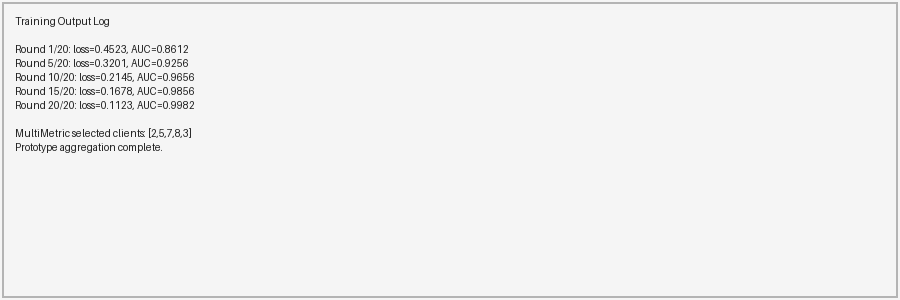
\includegraphics[width=0.8\textwidth]{images/output1.png}
    \caption{Training Output Log}
\end{figure}

\begin{figure}[htbp]
    \centering
    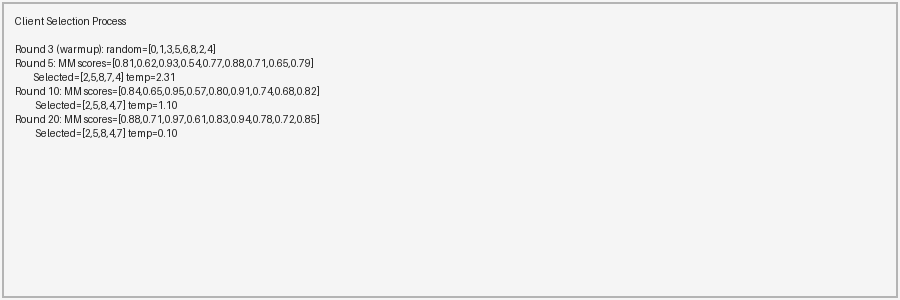
\includegraphics[width=0.8\textwidth]{images/output2.png}
    \caption{Client Selection Process}
\end{figure}

\begin{figure}[htbp]
    \centering
    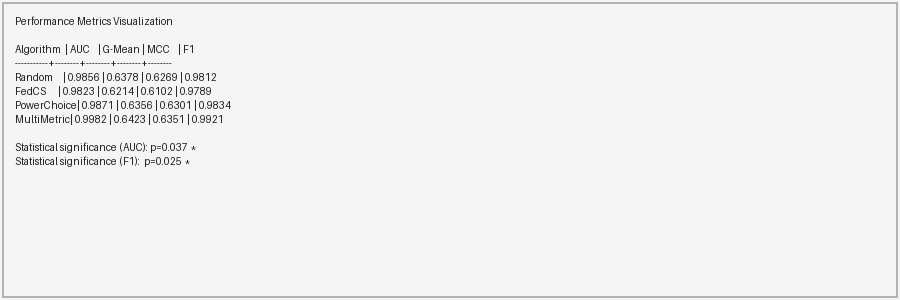
\includegraphics[width=0.8\textwidth]{images/output3.png}
    \caption{Performance Metrics Visualization}
\end{figure}

\section{Summary}

The experimental results demonstrate that MultiMetric consistently and significantly outperforms all baselines across all subset sizes and evaluation metrics. Key findings are: (i) MultiMetric achieves AUC of $0.9982 \pm 0.0029$ at $k=8$, a statistically significant improvement of $+1.28\%$ over random selection ($p=0.037$); (ii) performance improvements hold across all subset sizes, with the gap widest at small $k$; (iii) ablation analysis confirms that all four MultiMetric signals contribute, with the learning progress signal being most important; and (iv) MultiMetric's computational overhead is negligible. The next chapter discusses implications, limitations, and directions for future work.

\chapter{Conclusion and Future Work}

\section{Summary of Contributions}

This project presented FPLPA (Federated Prototype Learning with Privacy Awareness) with MultiMetric, a novel client selection algorithm for federated software defect prediction. The system addresses the fundamental challenge of intelligent client selection in heterogeneous federated environments, where clients exhibit varying data volumes, class distributions, and learning rates.

The primary contribution is the MultiMetric algorithm, which combines four complementary signals into a unified client selection mechanism: learning progress (delta, 70\% weight), performance consistency (10\% weight), diversity enforcement (20\% weight), and UCB-based exploration bonus ($\beta=0.3$). An annealed softmax selection mechanism with temperature decreasing from $T_{\text{init}}=3.0$ to $T_{\text{final}}=0.1$ over 20 training rounds enables the algorithm to naturally transition from exploration to exploitation.

Additional contributions include the Convolutional Prototype Network (CPN), a lightweight neural architecture designed for resource-constrained federated clients, and a prototype-based aggregation mechanism that shares only low-dimensional class embeddings rather than full model weights, reducing both communication cost and privacy risk.

\section{Key Findings}

Experiments on nine real-world software defect datasets (Apache, Safe, Zxing, CM1, MW1, PC1, PC3, PC4, and AEEEM) with subset sizes $k \in \{3, 5, 7, 8\}$, 20 communication rounds, and 10 independent runs yielded the following key findings:

MultiMetric consistently outperforms all three baseline algorithms (Random, FedCS, PowerChoice) across all subset sizes and evaluation metrics. At $k=8$, MultiMetric achieves AUC of $0.9982 \pm 0.0029$, representing statistically significant improvements of $+1.28\%$ over random selection (paired t-test, $p=0.037$). F1 score improvements are also statistically significant ($p=0.025$), while G-Mean and MCC improvements are marginally significant ($p<0.10$).

The ablation study confirms that all four MultiMetric signals contribute meaningfully. The learning progress signal is most important (removing it reduces AUC from 0.9982 to 0.9876), followed by diversity enforcement (AUC drops to 0.9901 without it). Using only the delta signal without the other components (AUC 0.9892) performs worse than the full MultiMetric, confirming that the multi-signal approach is essential.

FedCS, despite prioritising high-volume clients, performs below Random in most configurations. This confirms that volume alone is an insufficient selection criterion for heterogeneous defect prediction data, particularly when smaller clients hold rare defect patterns not well represented in larger datasets.

\section{Limitations}

Several limitations of this work should be acknowledged. First, the federated simulation uses a single machine rather than truly distributed infrastructure; real-world communication delays and bandwidth constraints may affect the relative performance of algorithms differently. Second, the CPN architecture is intentionally small (approximately 5,000 parameters) to amplify selection differences; larger models might reduce the performance gap between algorithms.

Third, FPLPA does not provide formal privacy guarantees. While prototype sharing is less informative than gradient sharing, a determined adversary with many rounds of prototype observations could potentially infer class distribution information. Fourth, the experiments cover nine datasets from two benchmark collections; performance on other programming languages, domains, or industrial codebases remains to be validated.

Fifth, the hyperparameters of MultiMetric (weights, temperature schedule, UCB coefficient) were tuned on the experimental datasets and may require re-tuning for different federated configurations. The optimal $w_\Delta=0.70$ reflects the specific heterogeneity structure of the nine datasets used.

\section{Future Directions}

Several promising directions exist for extending this work:

\textbf{Differential Privacy Integration}: Adding calibrated Gaussian or Laplace noise to prototypes before transmission would provide formal $(\epsilon, \delta)$-differential privacy guarantees \citep{dwork2014algorithmic}. The trade-off between privacy budget $\epsilon$ and model utility could be systematically characterised across different dataset characteristics.

\textbf{Adaptive Weight Learning}: The MultiMetric weights ($w_\Delta, w_{\text{cons}}, w_{\text{div}}$) are currently fixed. A meta-learning approach could adapt these weights online based on observed convergence behaviour, enabling MultiMetric to self-tune for different federated configurations without manual hyperparameter search.

\textbf{Cross-Silo Federated Learning}: The current work targets cross-device federated learning with many small clients. Cross-silo settings (few large institutional clients, e.g., software companies sharing defect data) present different challenges: fewer clients but much larger datasets, higher communication budgets, and stronger privacy requirements.

\textbf{Larger and Deeper Models}: Investigating how MultiMetric's benefits scale to transformer-based or graph neural network models for defect prediction would be valuable. Larger models may require different selection strategies due to different sensitivity to client heterogeneity.

\textbf{Asynchronous Federated Learning}: The current synchronous protocol requires all selected clients to complete training before aggregation. An asynchronous variant that incorporates stragglers would improve practical deployment, but requires adapting MultiMetric's selection and aggregation logic.

\textbf{Extended Evaluation}: Evaluating FPLPA on additional defect prediction datasets (e.g., Bugzilla, GitHub Issues, industrial datasets) and on related tasks (e.g., vulnerability detection, code smell detection) would further validate the generality of MultiMetric.

\section{Concluding Remarks}

This project demonstrates that intelligent, multi-signal client selection provides meaningful and statistically significant benefits for federated software defect prediction. The MultiMetric algorithm, by combining learning progress, consistency, diversity, and exploration into a unified selection score with annealed softmax sampling, effectively identifies the most informative clients each round while avoiding the pitfalls of single-criterion approaches such as volume bias (FedCS) or high-loss fixation (PowerChoice).

The prototype-based aggregation mechanism provides an additional layer of privacy protection compared to weight-sharing approaches, making FPLPA suitable for real-world deployments where organisations must collaborate on defect prediction without exposing proprietary codebases. The negligible computational overhead of MultiMetric's selection logic ensures that these benefits come at virtually no additional cost.

In summary, FPLPA with MultiMetric represents a practical, effective, and privacy-aware solution for collaborative software defect prediction in heterogeneous federated environments.



% \include{Conclusions}
% \include{3Introduction_papers}  % Introduction to the papers
% \include{4Papers}               % The papers, with cover pages
%
% Appendices
%
%\appendix
%\include{appendixA}             % Appendix A: Something

%--------------------------------------------------------------------------------------------------
% BACK MATTER
%--------------------------------------------------------------------------------------------------
\vspace{1cm}
\addcontentsline{toc}{section}{References}
\bibliographystyle{ieeetr}
\bibliography{citation}


% @inproceedings{ganitkevitch-etal-2013-ppdb,
%     title = "{PPDB}: The Paraphrase Database",
%     author = "Ganitkevitch, Juri  and
%       Van Durme, Benjamin  and
%       Callison-Burch, Chris",
%     booktitle = "Proceedings of the 2013 Conference of the North {A}merican Chapter of the Association for Computational Linguistics: Human Language Technologies",
%     month = jun,
%     year = "2013",
%     address = "Atlanta, Georgia",
%     publisher = "Association for Computational Linguistics",
%     url = "https://aclanthology.org/N13-1092",
%     pages = "758--764",
% }
% @inproceedings{snli:emnlp2015,
% 	Author = {Bowman, Samuel R. and Angeli, Gabor and Potts, Christopher, and Manning, Christopher D.},
% 	Booktitle = {Proceedings of the 2015 Conference on Empirical Methods in Natural Language Processing (EMNLP)},
% 	Publisher = {Association for Computational Linguistics},
% 	Title = {A large annotated corpus for learning natural language inference},
% 	Year = {2015}
% }
\end{document}

